%%%% supplementary_material_autodsc_2026.tex

\typeout{IJCAI--ECAI 26 Supplementary Material}

\documentclass[11pt]{article}
\usepackage[margin=1in]{geometry}

% Use the postscript times font!
\usepackage{times}
% \usepackage{soul}  % Not used
\usepackage{url}
\usepackage[hidelinks]{hyperref}
\usepackage[utf8]{inputenc}
\usepackage[small]{caption}
\usepackage{graphicx}
\usepackage{amsmath}
\usepackage{amsthm}
\usepackage{booktabs}
\usepackage{algorithm}
\usepackage{algpseudocode}
\usepackage{multirow}
\usepackage{array}
\usepackage{siunitx}
\usepackage{subcaption}
\usepackage{natbib}
\usepackage[switch]{lineno}

% Comment out this line in the camera-ready submission
\linenumbers

\urlstyle{same}

\setcounter{secnumdepth}{0} % No section numbers

\begin{document}

\title{AutoDD: Automated Drift Detector\\
\Large Supplementary Material}

\author{Anonymous}
\date{}

\maketitle

\appendix

\section{Additional Results}\label{appendix:additional_results}

This section presents additional experimental analysis using Hoeffding Adaptive Tree (HAT) as the base classifier, demonstrating that AutoDD's performance generalizes across different base classifiers.

\textbf{Statistical Significance:} Figure~\ref{fig:cd_hat} shows the Critical Difference diagram based on Friedman test with Nemenyi post-hoc analysis across all methods using HAT as the base classifier. AutoDD achieves the best average rank, significantly outperforming all fixed detectors and ranking substantially better than state-of-the-art methods.

\textbf{Computational Efficiency:} Figure~\ref{fig:time_memory_hat} compares runtime and memory across methods using HAT as the base classifier. AutoDD maintains competitive efficiency, being significantly faster than Meta-ADD while achieving higher accuracy and maintaining classical detector-level computational overhead while achieving state-of-the-art performance.

\begin{figure}[ht]
\centering
\begin{subfigure}[b]{0.48\textwidth}
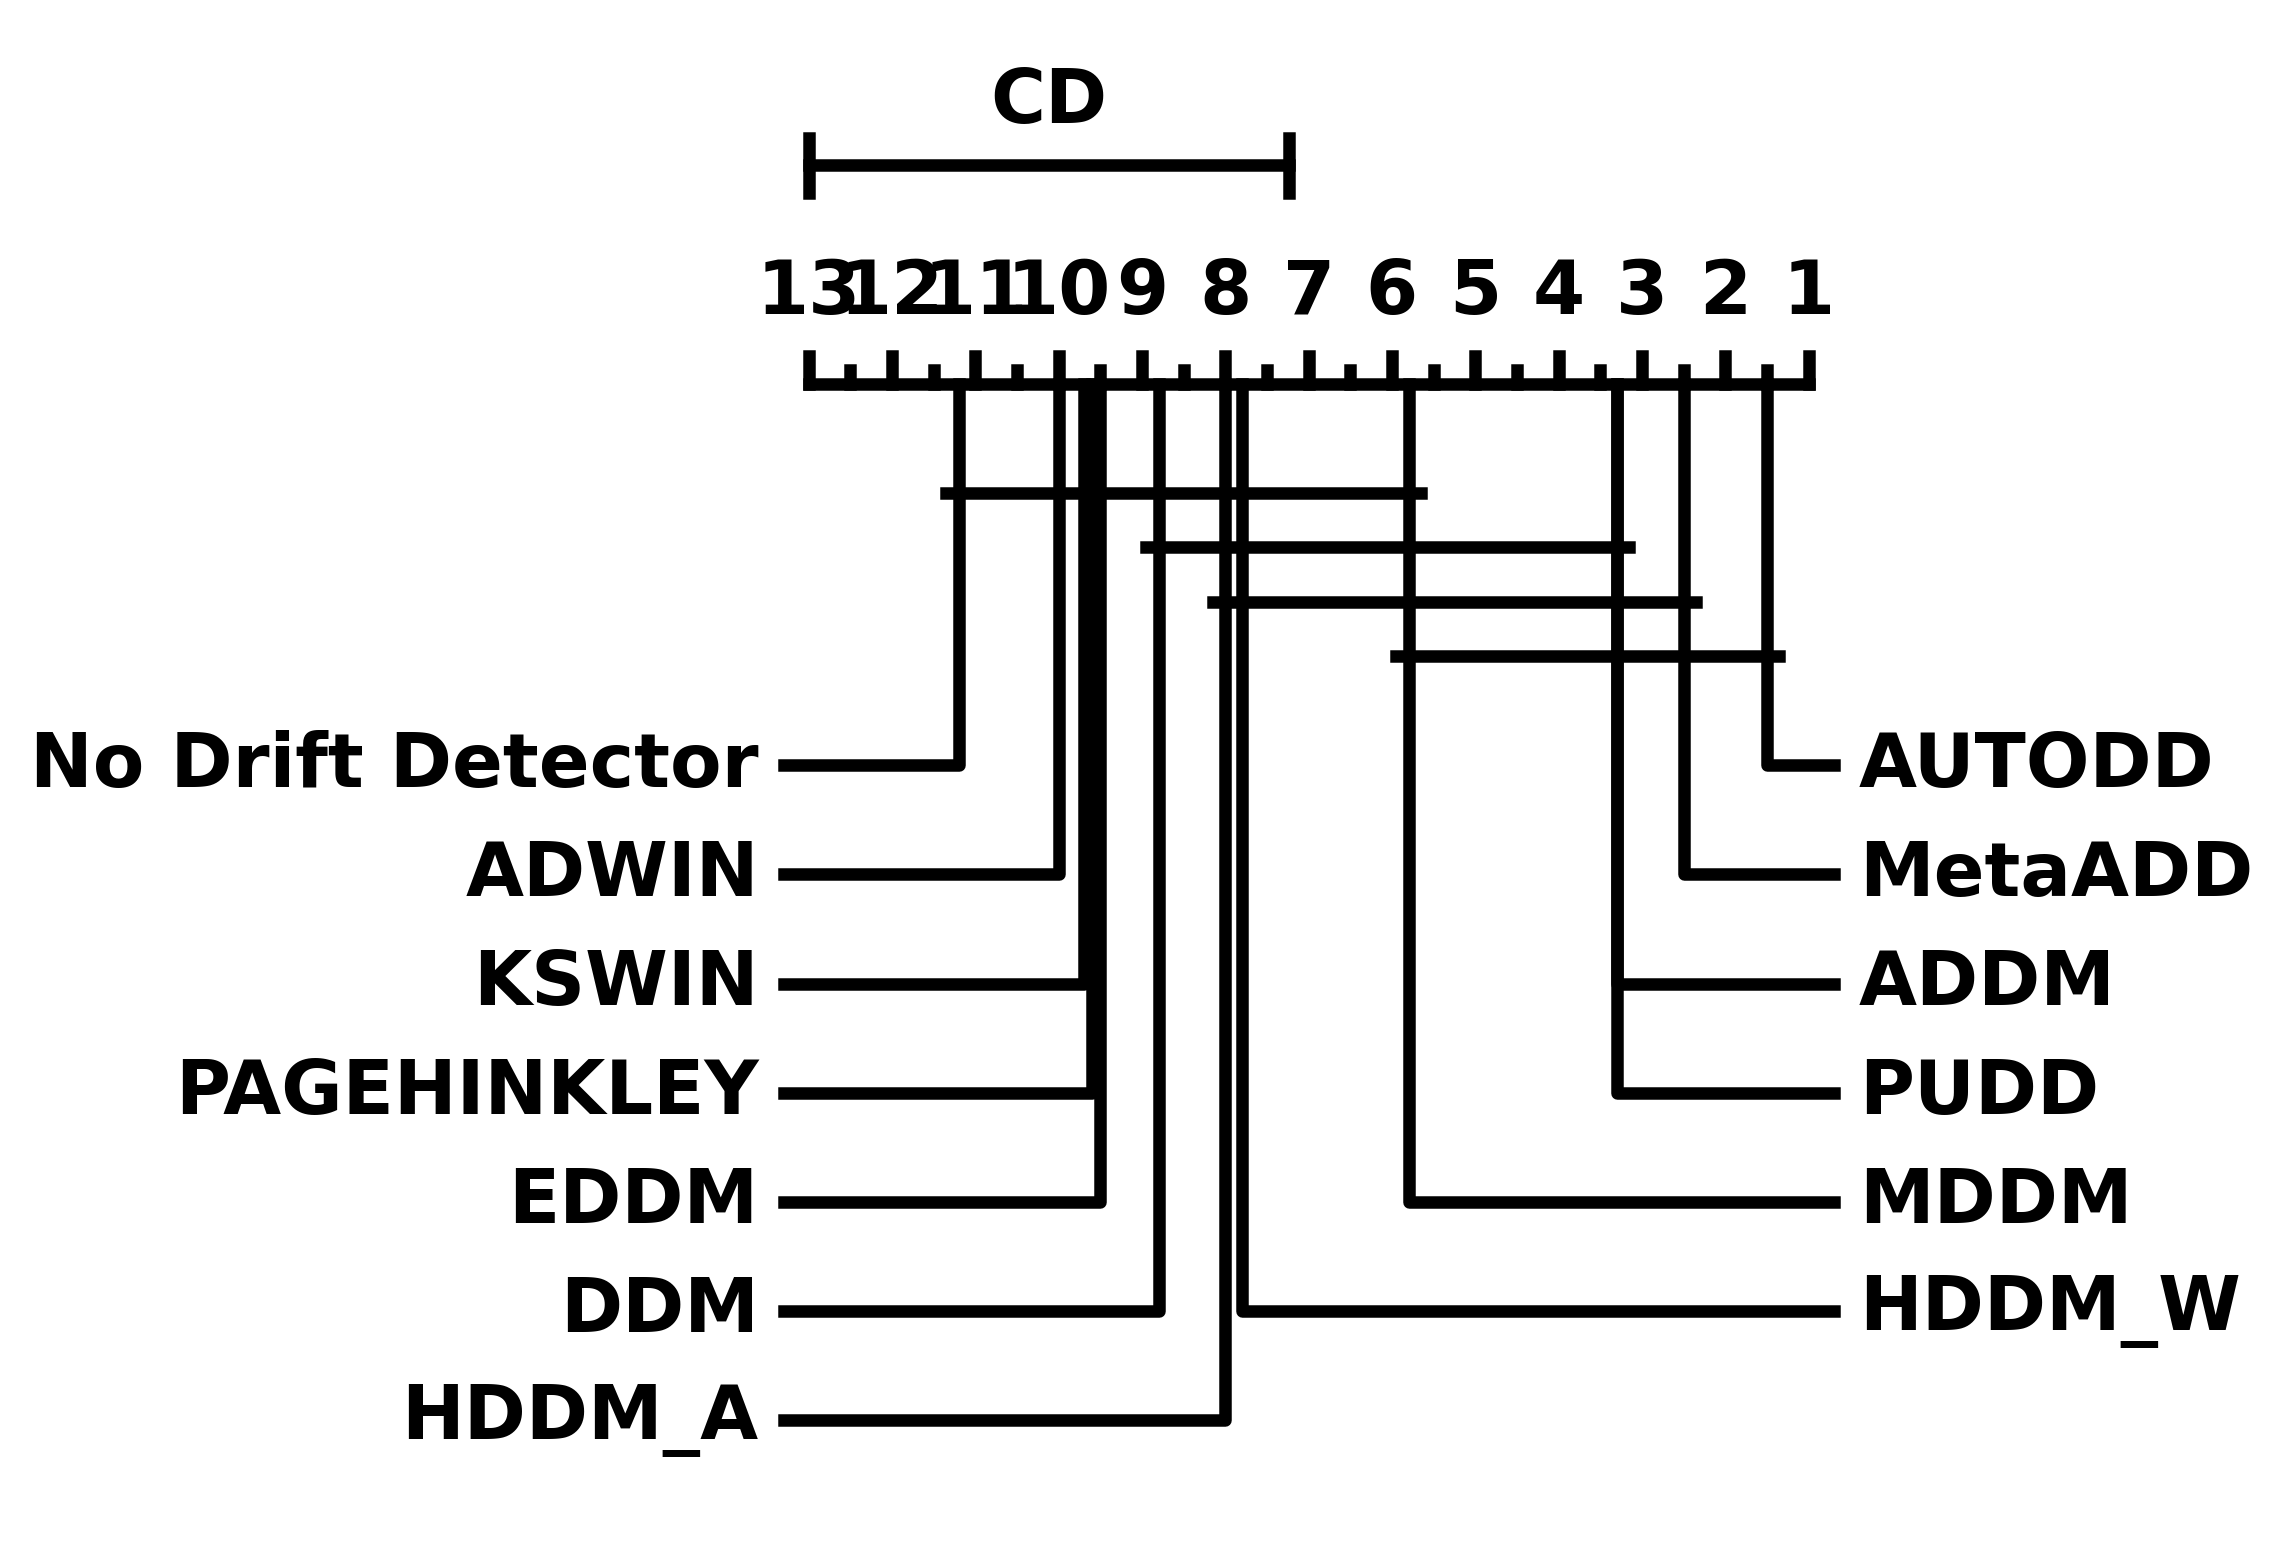
\includegraphics[width=\textwidth]{images_supply/cd_diagram_hat.png}
\caption{Critical Difference diagram}
\label{fig:cd_hat}
\end{subfigure}
\hfill
\begin{subfigure}[b]{0.48\textwidth}
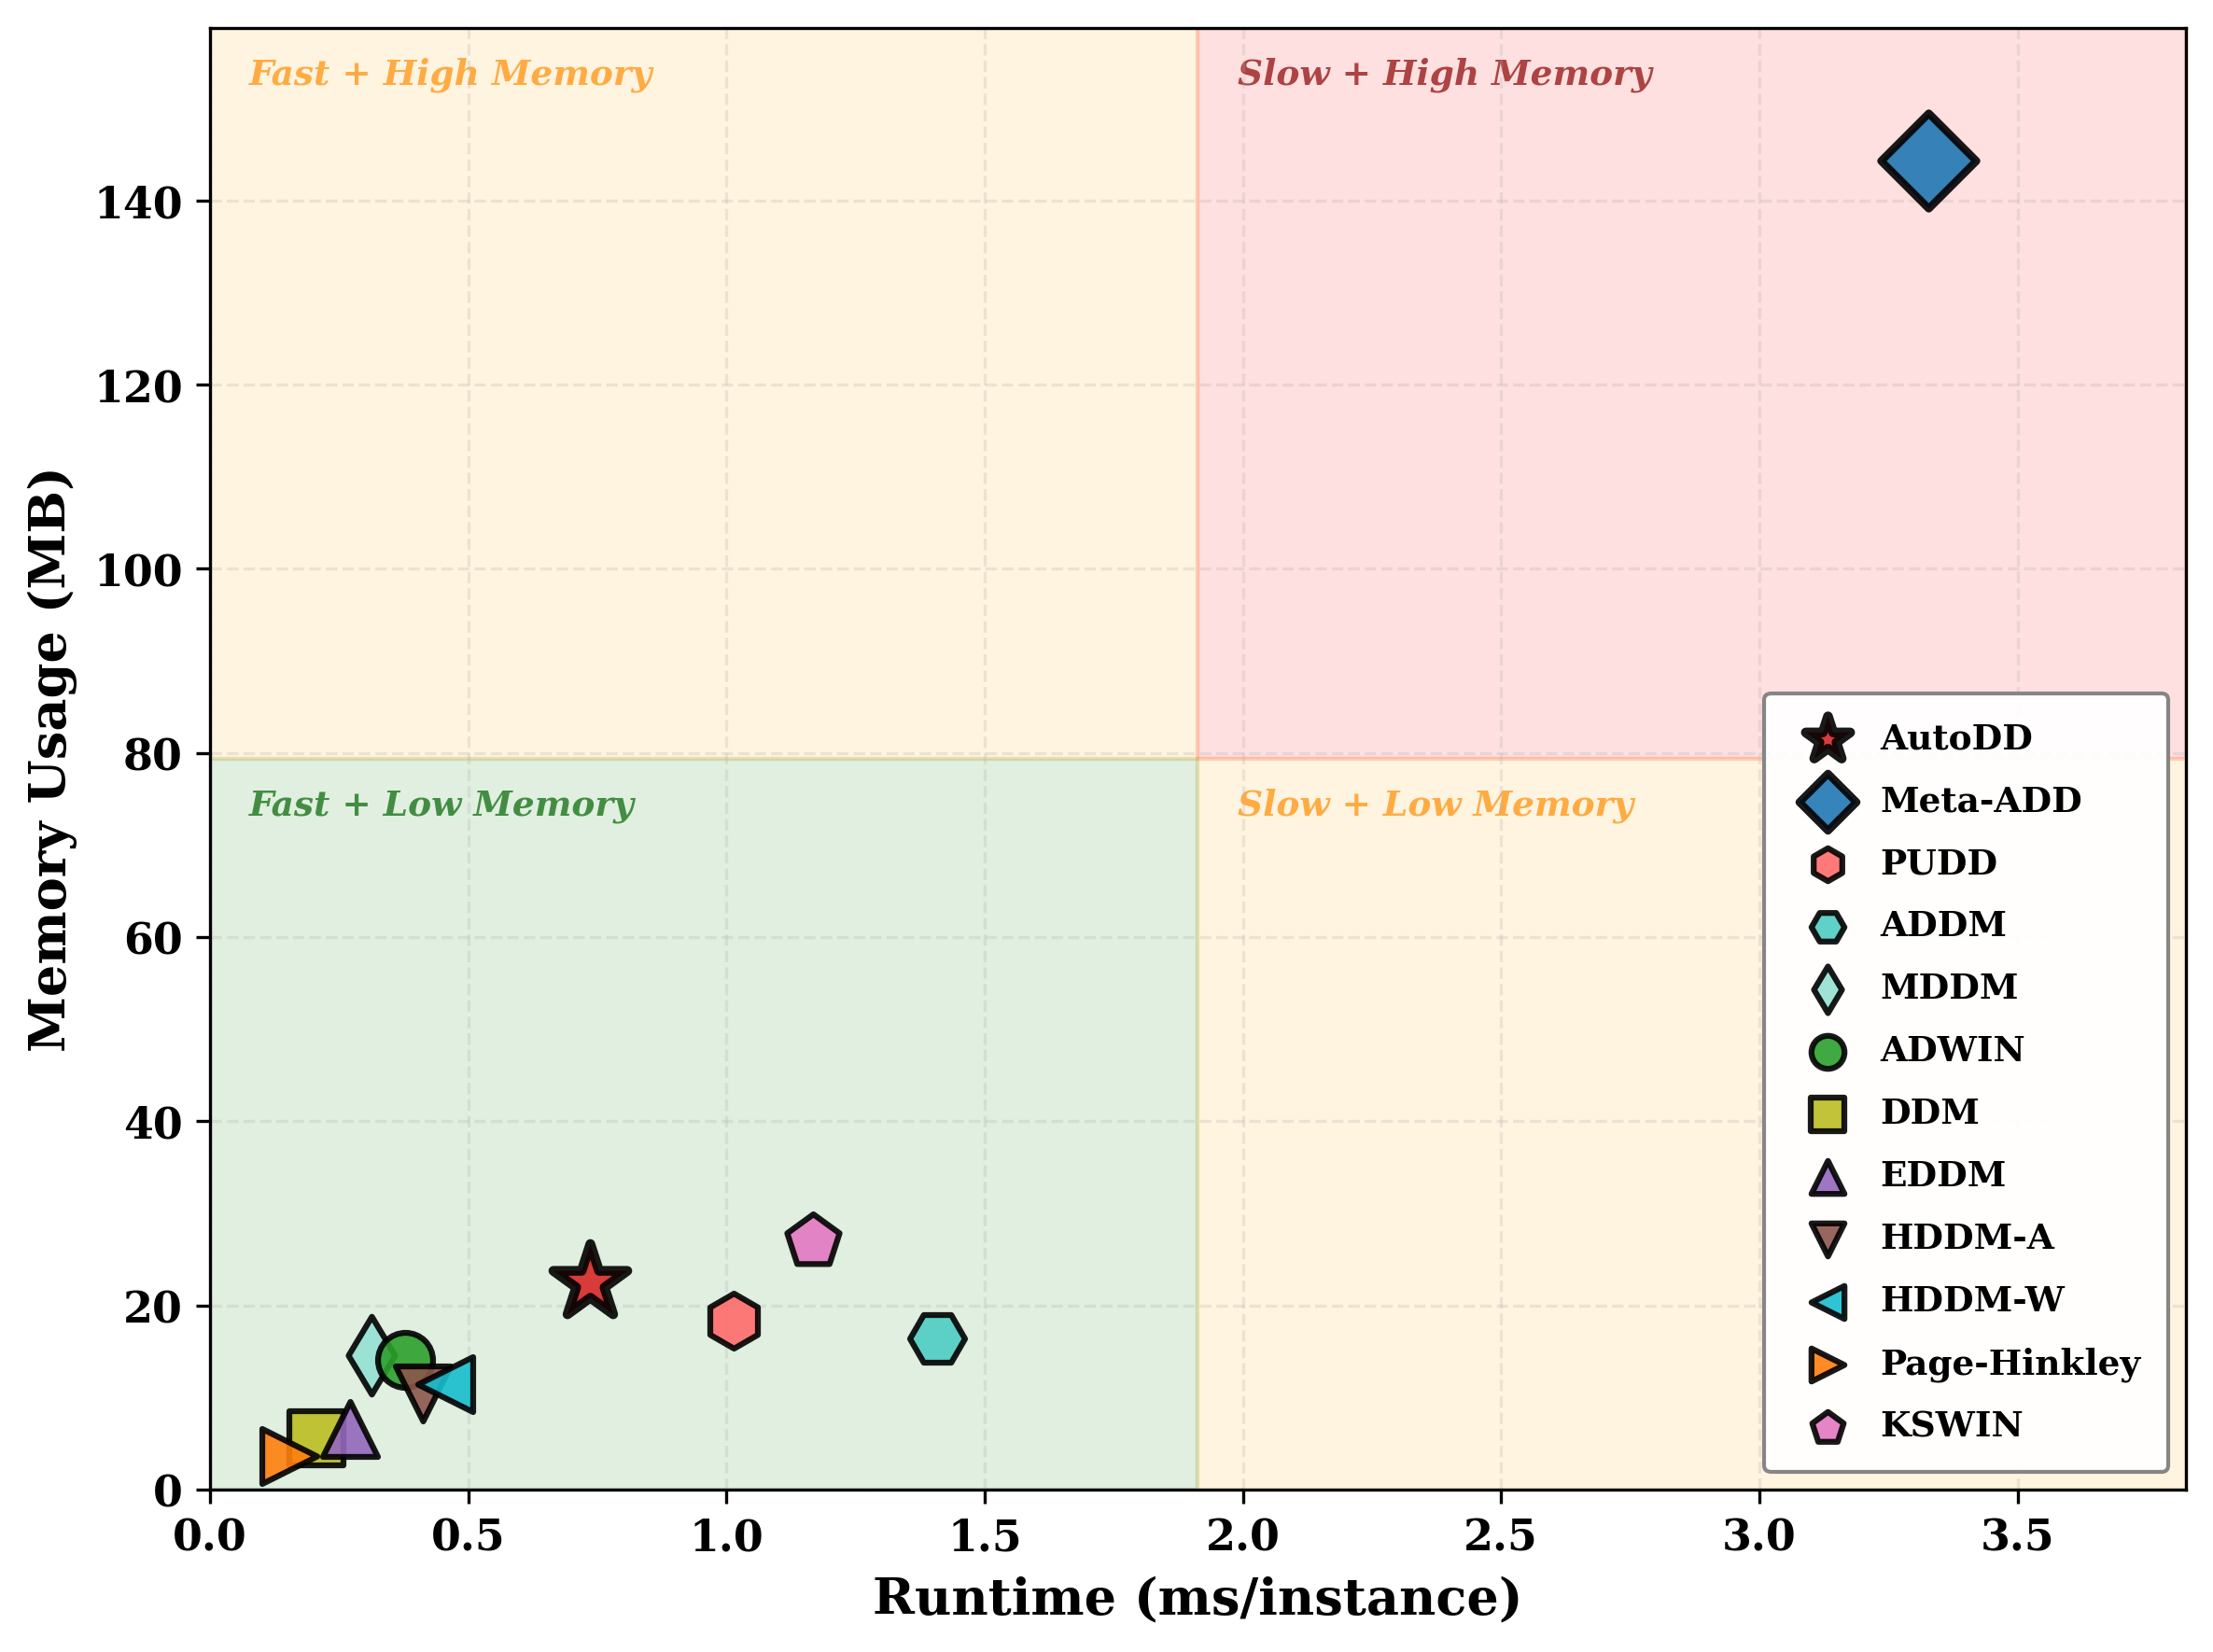
\includegraphics[width=\textwidth]{images_supply/time_memory_hat.png}
\caption{Runtime vs. memory trade-off}
\label{fig:time_memory_hat}
\end{subfigure}
\caption{Statistical significance analysis and computational efficiency with HAT base classifier. (a) Critical Difference diagram with connecting bars indicating statistically equivalent methods ($\alpha=0.05$). (b) Runtime vs. memory trade-off showing AutoDD achieves the best accuracy while maintaining reasonable computational overhead.}
\label{fig:stats_efficiency}
\end{figure}

\bibliographystyle{named}
\bibliography{references}

\end{document}
